\documentclass[11pt]{article}
\title{Symmetry 9}
\author{https://github.com/heptagons/lenses}
\date{2024/1/16}

\usepackage{graphicx}

\usepackage[margin=0.75in]{geometry}
\usepackage{float} % {figure}{H}
\usepackage{amsmath} % \dfrac

\def\mathbi#1{\textbf{\em #1}}

\begin{document}

\maketitle
\begin{abstract}
We build equilateral polygons that can tesselate the plane using the symmetry $9$. We analyze lower odd symmetries $3,5,7$ also to find patterns. The polygons are rhombus, hexagons, octagons and stars.
\end{abstract}

\section{Symmetries}

We are interested in odd symmetries starting with $3$. Table \ref{tbl:symm} show the symmetries up to $9$. The value of the angle of the symmetry $m$ is $\theta = \dfrac{2\pi}m$. 

\begin{table}[H]
\begin{center}
\begin{tabular}{|c|c c|}
\hline
$m$ & Angle & $\theta$ \\ \hline\
$3$ & $\alpha$ & $2\pi/3$ \\ \hline
$5$ & $\beta$  & $2\pi/5$ \\ \hline
$7$ & $\gamma$ & $2\pi/7$ \\ \hline
$9$ & $\delta$ & $2\pi/9$ \\ \hline
\end{tabular}
\caption{Symmetries $m=\{3,5,7,9\}$.} 
\label{tbl:symm}
\end{center}
\end{table}

\section{Rhombi}

Rhombi are equilateral tetragons. For every odd symmetry $m$ we find $n = \dfrac{m-1}2$ different rhombi. The rhombi smallest angles are defined as $\omega_1 \equiv \dfrac{i}2$ while the other as $\omega_2 \equiv n + \dfrac{i-1}2$ where $i = 1,...,n$. We identify the rhombi with the symmetry $m$ and angle $\omega_1$ only. So for symmetry $9$ we have the four rhombi: $R_9\left(\frac{1}2\right)$, $R_9(1)$, $R_9\left(\frac{3}2\right)$ and $R_9(2)$.

Figure \ref{tbl:rhombi} show the rhombi for symmetries up to $9$. Every rhombus is labeled with a consecutive lowercase letter $\mathbi{a}$, $\mathbi{b}$, $\mathbi{c}$,... The first rhombi $\mathbi{a}$ is found again in symmetry $9$ so we prevent renaming identical rhombi.

The rhombi angles $\theta_1$ and $\theta_2$ are expressed in function of the angles $\{\alpha,\beta,\gamma,\delta\}$ of symmetries $m=\{3,5,7,9\}$ where $\theta_1 < \theta_2$ and $\theta_1 + \theta_2 = \pi$. We cannot use the rhombi isolated in our tessellations since not both $\omega_1$ and $\omega_2$ are integers. But we'll add and substract rhombi together to build hexagons, octagons and beyond where all polygon's angles $\omega_n$ are integers.

\begin{table}[h]
\begin{center}
\begin{tabular}{|c|c|c|c c| r |}
\hline
$R_m(\omega_1)$ & $\omega_2$ & Name & $\theta_1$ & $\theta_2$ & Area \\ \hline\
$R_3(\frac{1}2)$ & $1$  & $\mathbi{a}$ & $\alpha/2$ & $2\alpha/2$  & $\sin(\alpha) \approx 0.866$ \\[0.5ex]
\hline
$R_5(\frac{1}2)$ & $2$  & $\mathbi{b}$ & $\beta/2$  & $4\beta/2$   & $\sin(2\beta) \approx 0.587$\\[0.5ex]
$R_5(1)$ & $\frac{3}2$  & $\mathbi{c}$ & $2\beta/2$ & $3\beta/2$   & $\sin(\beta) \approx 0.951$\\[0.5ex]
\hline
$R_7(\frac{1}2)$ & $3$  & $\mathbi{d}$ & $\gamma/2$ & $6\gamma/2$  & $\sin(3\gamma) \approx 0.433$\\[0.5ex]
$R_7(1)$ & $\frac{5}2$ & $\mathbi{e}$ & $2\gamma/2$ & $5\gamma/2$ & $\sin(\gamma) \approx 0.781$\\[0.5ex]
$R_7(\frac{3}2)$ & $2$  & $\mathbi{f}$ & $3\gamma/2$ & $4\gamma/2$ & $\sin(2\gamma) \approx 0.974$\\[0.5ex]
\hline
$R_9(\frac{1}2)$ & $4$ & $\mathbi{g}$ & $\delta/2$ & $8\delta/2$  & $\sin(4\delta) \approx 0.342$\\[0.5ex]
$R_9(1)$ & $\frac{7}2$ & $\mathbi{h}$ & $2\delta/2$ & $7\delta/2$ & $\sin(\delta) \approx 0.642$\\[0.5ex]
$R_9(\frac{3}2)$ & $3$ & $\mathbi{a}$ & $3\delta/2$ & $6\delta/2$ & $\sin(3\delta) \approx 0.866$\\[0.5ex]
$R_9(2)$ & $\frac{5}2$ & $\mathbi{i}$ & $4\delta/2$ & $5\delta/2$ & $\sin(2\delta) \approx 0.984$\\[0.5ex]
\hline
\end{tabular}
\caption{Rhombi $R_m(\omega_1,\omega_2)$ for symmetries $m=\{3,5,7,9\}$.} 
\label{tbl:rhombi}
\end{center}
\end{table}

\section{Stars}

For every odd symmetry $m$ we have several stars that are equilateral 2$m$-gons with at most two different angles $\omega_1$ and $\omega_2$ at the vertices. We find exactly $n = \dfrac{m-1}2$ different stars with angles $\omega_1 \leq \omega_2$ as integers.

Figure \ref{tbl:stars} show the stars for symmetries up to $9$. Every star with both $\omega_1$ and $\omega_2$ integers are labeled with a consecutive uppercase letter $\mathcal{A}, \mathcal{B}, \mathcal{C}...$. The stars are easily build with rhombi so the table show the stars area in function of them.

\begin{table}[H]
\begin{center}
\begin{tabular}{|c|c|c|l|l|}
\hline
$S_m(\omega_1)$ & $\omega_2$ & Name & Area & Polygon \\ \hline\
$S_3(\frac{1}2)$ & $2$ & -     & $6\mathbi{a}$ & $|6/2|$ (12-gon) \\[0.5ex]
$S_3(1)$         & $1$ & $\mathcal{A}$ & $3\mathbi{a}$ & Regular hexagon \\[0.5ex]
\hline
$S_5(\frac{1}2)$ & $4$ & -      & $5\mathbi{b}$ & $|10/4|$ (20-gon)\\[0.5ex]
$S_5(1)$ & $3$ & $\mathcal{B}$ & $5\mathbi{c}$ & $|(5/2)_\alpha|$ decagram\\[0.5ex]
$S_5(2)$ & $2$ & $\mathcal{C}$ & $5(\mathbi{c}+\mathbi{b})$ & Regular decagon\\[0.5ex]
\hline
$S_7(\frac{1}2)$ & $6$ & -     & $7\mathbi{d}$ & $|14/6|$ (28-gon)\\[0.5ex]
$S_7(1)$ & $5$ & $\mathcal{D}$ & $7\mathbi{e}$ & $|(7/4)_\alpha|$ 14-gram\\[0.5ex]
$S_7(2)$ & $4$ & $\mathcal{E}$ & $7(\mathbi{e}+\mathbi{f})$ & $|(7/2)_\alpha|$ 14-gram\\[0.5ex]
$S_7(3)$ & $3$ & $\mathcal{F}$ & $7(\mathbi{e}+\mathbi{f}+\mathbi{d})$ & Regular 14-gon\\[0.5ex]
\hline
$S_9(\frac{1}2)$ & $8$ & -     & $9\mathbi{g}$ & $|18/8|$ (36-gon)\\[0.5ex]
$S_9(1)$ & $7$ & $\mathcal{G}$ & $9\mathbi{h}$ & $|(9/6)_\alpha|$ 18-gram\\[0.5ex]
$S_9(2)$ & $6$ & $\mathcal{H}$ & $9(\mathbi{h}+\mathbi{i})$ & $|(9/4)_\alpha|$ 18-gram\\[0.5ex]
$S_9(3)$ & $5$ & $\mathcal{I}$ & $9(\mathbi{h}+\mathbi{i}+\mathbi{a})$ & $|(9/2)_\alpha|$ 18-gram\\[0.5ex]
$S_9(4)$ & $4$ & $\mathcal{J}$ & $9(\mathbi{h}+\mathbi{i}+\mathbi{a}+\mathbi{g})$ & Regular 18-gon\\[0.5ex]
\hline
\end{tabular}
\caption{Stars $S_m(\omega_1,\omega_2)$ for symmetries $m=\{3,5,7,9\}$.}
\label{tbl:stars}
\end{center}
\end{table}

Figure \ref{fig:rhombi-9} show nine copies of symmetry-9 rhombi $\{\mathbi{h},\mathbi{i},\mathbi{a},\mathbi{g}\}$ forming the four stars $S_9(1)$, $S_9(2)$, $S_9(3)$ and $S_9(4)$ named respectivelly $\mathcal{G}$, $\mathcal{H}$, $\mathcal{I}$ and $\mathcal{J}$.

\begin{figure}[H]
\centering
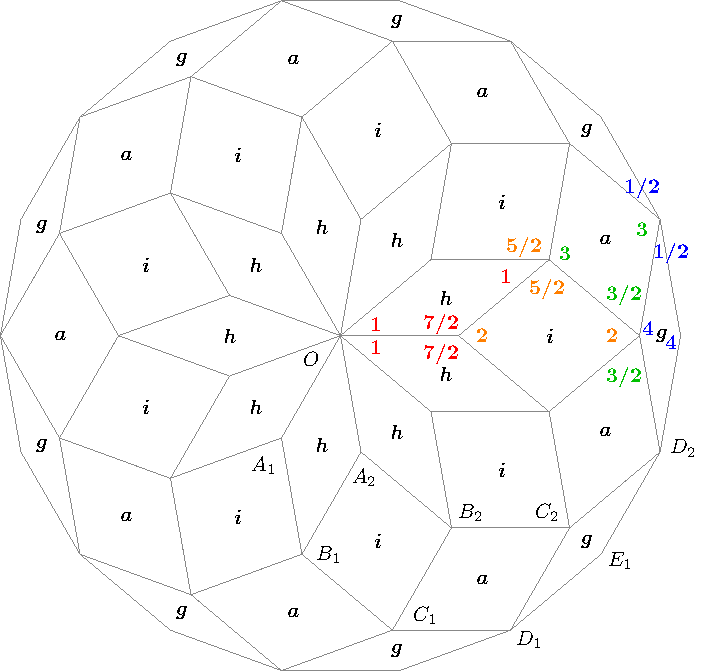
\includegraphics[scale=1]{rhombi-9}
\caption{The symmetry $9$ four rhombi $\{\mathbi{h},\mathbi{i},\mathbi{a},\mathbi{g}\}$ produce the four stars $\{\mathcal{G},\mathcal{H},\mathcal{I},\mathcal{J}\}$ with areas
$9\mathbi{h}$,
 $9(\mathbi{h}+\mathbi{i})$,
 $9(\mathbi{h}+\mathbi{i}+\mathbi{a})$ and 
 $9(\mathbi{h}+\mathbi{i}+\mathbi{a}+\mathbi{g})$ respectivelly.}
\label{fig:rhombi-9}
\end{figure}





\section{Hexagons}

For any odd symmetry $m$, we can obtain equilateral hexagons by connecting six equal edges at integral values of $\omega$ or by adding and substracting rhombi or by dissecting the areas left after stars intersections. In any case we find the hexagons has at most three different internal angles in this order $(\omega_1, \omega_2, \omega_3, \omega_1, \omega_2, \omega_3)$ where $\omega_1 + \omega_2 + \omega_3 = m$.

\subsection{Hexagons angles}


Figure \ref{tbl:hexagons-angles} show the hexagons defined as $H_m(\omega_1,\omega_2)$ for symmetries $m = \{3,5,7,9\}$ where $\omega_1 \leq \omega_2 \leq \omega_3$. We labeled the non self-intersecting hexagons with uppercase letters $\mathbi{A}$, $\mathbi{B}$, $\mathbi{C}$, ... We prevent to name differently any hexagon which is equivalent to a previous one having the same angles as what happens with hexagon $\mathbi{A}$ of symmetries $3$ and $9$.

\begin{table}[H]
\begin{center}
\begin{tabular}{| c | c | c | l | }
\hline
$H_m(\omega_1,\omega_2)$ & Name & $(\omega_1, \omega_2, \omega_3)$ & Polygon \\ \hline\
$H_3(1,1)$ & \mathbi{A} & (\textbf{1, 1, 1}) & Regular hexagon \\[0.5ex]
\hline
$H_5(1,1)$ & \mathbi{B} & (\textbf{1, 1, 3}) & Sormeh Dan Girih tile\\[0.5ex]
$H_5(1,2)$ & \mathbi{C} & (\textbf{1, 2, 2}) & Shesh Band Girih tite\\[0.5ex]
\hline
$H_7(1,1)$ & -          & (\textbf{1, 1, 5}) & self-intersecting \\[0.5ex]
$H_7(1,2)$ & \mathbi{D} & (\textbf{1, 2, 4}) & \\[0.5ex]
$H_7(1,3)$ & \mathbi{E} & (\textbf{1, 3, 3}) & \\[0.5ex]
$H_7(2,2)$ & \mathbi{F} & (\textbf{2, 2, 3}) & \\[0.5ex]
\hline
$H_9(1,1)$ & -          & (\textbf{1, 1, 7}) & self-intersecting \\[0.5ex]
$H_9(1,2)$ & \mathbi{G} & (\textbf{1, 2, 6}) & \\[0.5ex]
$H_9(1,3)$ & \mathbi{H} & (\textbf{1, 3, 5}) & \\[0.5ex]
$H_9(1,4)$ & \mathbi{I} & (\textbf{1, 4, 4}) & \\[0.5ex]
$H_9(2,2)$ & \mathbi{J} & (\textbf{2, 2, 5}) & \\[0.5ex]
$H_9(2,3)$ & \mathbi{K} & (\textbf{2, 3, 4}) & \\[0.5ex]
$H_9(3,3)$ & \mathbi{A} & (\textbf{3, 3, 3}) & equivalent to $H_3(1,1)$\\[1.1ex]
\hline
\end{tabular}
\caption{Hexagons $H_m(\omega_1,\omega_2)$ for symmetries $m = \{3,5,7,9\}$.} 
\label{tbl:hexagons-angles}
\end{center}
\end{table}


\subsection{Hexagons areas}

\begin{figure}[H]
\centering
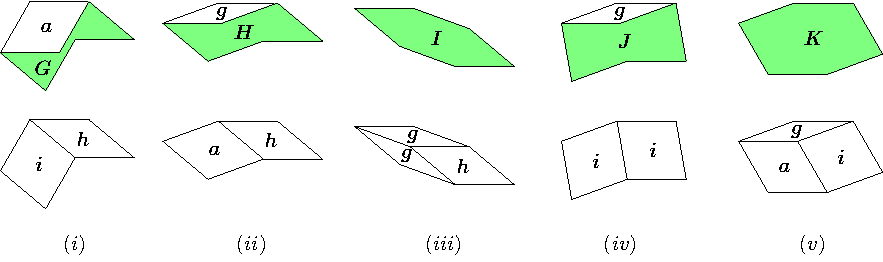
\includegraphics[scale=1]{hexagons-from-rhombi-9}
\caption{Symmetry $9$ hexagons formed adding and substracting rhombi.}
\label{fig:hexagons-from-rhombi-9}
\end{figure}

Figure \ref{fig:hexagons-from-rhombi-9} show how to calculate the area of the symmetry $9$ hexagons in function of the symmetry $9$ rhombi. From $(i)$ to $(vi)$ we equate the area of sum of the polygons in the top with the area of the sum of the polygons of the bottom. We have for the six cases these six equations:
\begin{align}
\mathbi{a} + \mathbi{G} &= \mathbi{i} + \mathbi{h} \\
\mathbi{g} + \mathbi{H} &= \mathbi{a} + \mathbi{h} \\
\mathbi{I} &= 2\mathbi{g} + \mathbi{h} \\
\mathbi{g} + \mathbi{J} &= 2\mathbi{i} \\
\mathbi{K} &= \mathbi{g} + \mathbi{a} + \mathbi{i} \\
\mathbi{A} &= 3\mathbi{a}
\end{align}

\begin{figure}[H]
\centering
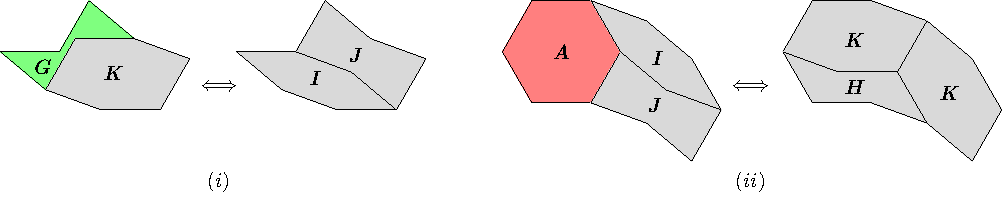
\includegraphics[scale=1]{hexagons-from-hexagons-9}
\caption{Hexagons $\{\mathbi{G},\mathbi{A}\}$ formed adding and substracting hexagons $\{\mathbi{H},\mathbi{I},\mathbi{J},\mathbi{K}\}$.}
\label{fig:hexagons-from-hexagons-9}
\end{figure}

Figure \ref{fig:hexagons-from-hexagons-9} show how to express the area of the six hexagons in function of only four. For $(i)$ and $(ii)$ we equate the area of the sum of hexagons of the left with the area of the hexagons of the right. We have for the two cases these two equations:
\begin{align}
\mathbi{G} + \mathbi{K} &= \mathbi{I} + \mathbi{J} \\
\mathbi{A} + \mathbi{I} + \mathbi{J} &= \mathbi{H} + 2\mathbi{K}
\end{align}

Using the last eight equations we form the table \ref{tbl:hexagons-areas} which show the areas of the six hexagons in function of four rhombi $\mathbi{g,h,a,i}$ and in function of only four hexagons $\mathbi{H,I,J,K}$.

\begin{table}[H]
\begin{center}
\begin{tabular}{| c | l | l |}
\hline
Hexagon & $\mathbi{g,h,a,i}$ area & $\mathbi{H,I,J,K}$ area \\ \hline\
$\mathbi{H}$ & $\mathbi{a} + \mathbi{h} - \mathbi{g}$ & $\mathbi{H}$ \\[0.5ex]
$\mathbi{I}$ & $2\mathbi{g} + \mathbi{h}$ & $\mathbi{I}$ \\[0.5ex]
$\mathbi{J}$ & $2\mathbi{i} - \mathbi{g}$ & $\mathbi{J}$ \\[0.5ex]
$\mathbi{K}$ & $\mathbi{g} + \mathbi{a} + \mathbi{i}$ & $\mathbi{K}$ \\[0.5ex]
\hline
$\mathbi{A}$ & $3\mathbi{a}$ & $2\mathbi{K} + \mathbi{H} - \mathbi{I} - \mathbi{J}$ \\[0.5ex]
$\mathbi{G}$ & $\mathbi{i} + \mathbi{h} - \mathbi{a}$ & $\mathbi{I} + \mathbi{J} - \mathbi{K}$ \\[0.5ex]
\hline
\end{tabular}
\caption{Symmetry $9$ hexagon areas.} 
\label{tbl:hexagons-areas}
\end{center}
\end{table}


\subsection{Hexagons from stars}

Figure \ref{fig:hexagons-9} show the disposition of the symmetry $9$ four stars. We label the $18$ vertices of stars $\{\mathcal{G},\mathcal{H},\mathcal{I},\mathcal{J}\}$ as
 $\{G_0,G_1,...,G_{17}\}$,
 $\{H_0,H_1,...,H_{17}\}$,
 $\{I_0,I_1,...,I_{17}\}$ and
 $\{I_0,G_1,...,I_{17}\}$ respectivelly. 
For simplicity, only some vertices are show. First we make coincident at vertice $O$ all the vertices $G_0,H_0,I_0,J_0$. With the center at $O$ we rotate all stars to make coincidents
$G_{17}$, $H_{17}$, $I_{17}$ and $J_{17}$. The rotations also joined another different vertices.

First we add three new edges (in red) joining the stars $\mathcal{J}$ and $\mathcal{I}$ vertices: $\overline{J_3I_2}$, $\overline{J_5I_4}$ and $\overline{J_7I_6}$ dissecting the red region into four hexagons, two of them essentially different. The three consective angles of the two hexagons are shown: $\textbf{I (1,4,4)}$ and $\textbf{K (3,4,2)}$.

Then we add three new edges (in orange) joining the stars $\mathcal{I}$ and $\mathcal{H}$ vertices: $\overline{I_3H_2}$, $\overline{I_5H_4}$ and $\overline{I_7H_6}$ dissecting the orange region into four hexagons, two of them new. The three consective angles of the the two hexagons are show: $\textbf{H (1,5,3)}$ and $\textbf{A (3,3,3)}$.

Finally we add three more edges (in green) joining the stars $\mathcal{H}$ and $\mathcal{G}$ vertices:
$\overline{H_3G_2}$, $\overline{H_5G_4}$ and $\overline{H_7G_6}$ dissecting the green region into four hexagons, two of them new. The three consective angles of the the two hexagons are show: $\textbf{G (1,6,2)}$ and $\textbf{J (2,5,2)}$.


\begin{figure}[H]
\centering
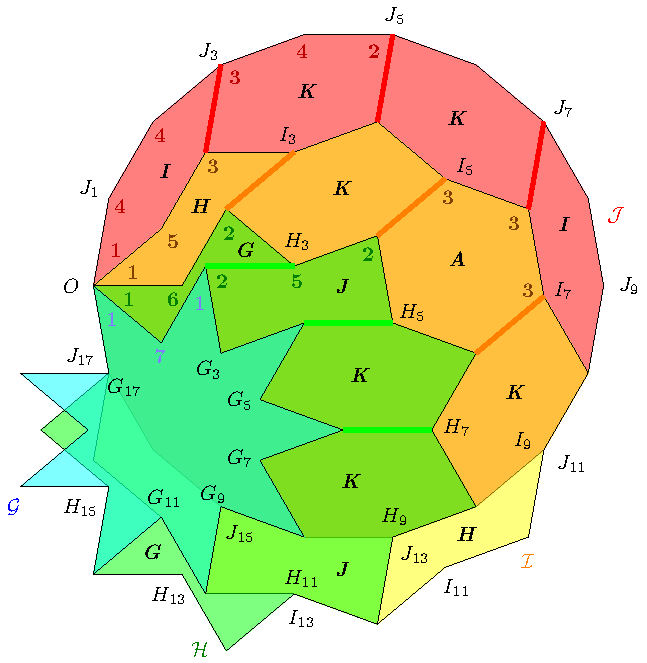
\includegraphics[scale=1]{hexagons-9}
\caption{Symmetry $9$ stars $\{\mathcal{G},\mathcal{H},\mathcal{I},\mathcal{J}\}$
 dissected to get the six hexagons
$\{\mathbi{G},\mathbi{H},\mathbi{I},\mathbi{J},\mathbi{K},\mathbi{A}\}$.
}
\label{fig:hexagons-9}
\end{figure}

\section{Octagons}

\subsection{Octagons by stars}

\begin{figure}[H]
\centering
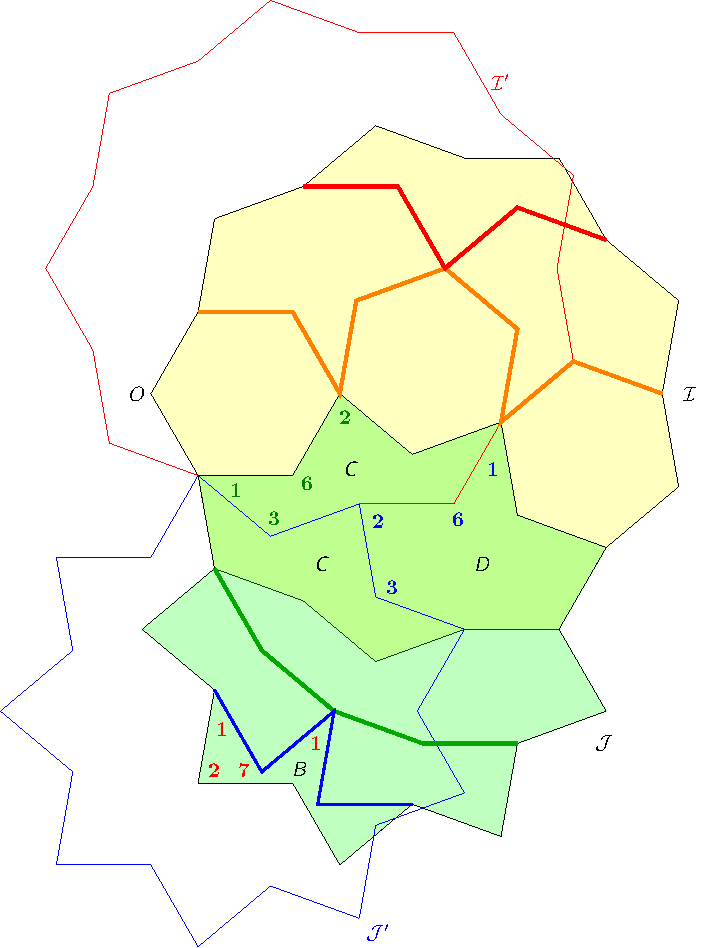
\includegraphics[scale=1]{octagons-9}
\caption{Octagons after intersection of stars $\mathcal{I}$ and $\mathcal{J}$.}
\label{fig:octagons-9}
\end{figure}



\end{document}

